%%%%%%%%%%%%%%%%%%%%%%%%%%%%%%%%%%%%%%%%%
% Arsclassica Article
% LaTeX Template
% Version 1.1 (1/8/17)
%
% This template has been downloaded from:
% http://www.LaTeXTemplates.com
%
% Original author:
% Lorenzo Pantieri (http://www.lorenzopantieri.net) with extensive modifications by:
% Vel (vel@latextemplates.com)
%
% License:
% CC BY-NC-SA 3.0 (http://creativecommons.org/licenses/by-nc-sa/3.0/)
%
%%%%%%%%%%%%%%%%%%%%%%%%%%%%%%%%%%%%%%%%%

%----------------------------------------------------------------------------------------
%	PACKAGES AND OTHER DOCUMENT CONFIGURATIONS
%----------------------------------------------------------------------------------------

\documentclass[
10pt, % Main document font size
letterpaper, % Paper type, use 'letterpaper' for US Letter paper
oneside, % One page layout (no page indentation)
%twoside, % Two page layout (page indentation for binding and different headers)
headinclude,footinclude, % Extra spacing for the header and footer
BCOR5mm, % Binding correction
]{scrartcl}

%%%%%%%%%%%%%%%%%%%%%%%%%%%%%%%%%%%%%%%%%
% Arsclassica Article
% Structure Specification File
%
% This file has been downloaded from:
% http://www.LaTeXTemplates.com
%
% Original author:
% Lorenzo Pantieri (http://www.lorenzopantieri.net) with extensive modifications by:
% Vel (vel@latextemplates.com)
%
% License:
% CC BY-NC-SA 3.0 (http://creativecommons.org/licenses/by-nc-sa/3.0/)
%
%%%%%%%%%%%%%%%%%%%%%%%%%%%%%%%%%%%%%%%%%

%----------------------------------------------------------------------------------------
%	REQUIRED PACKAGES
%----------------------------------------------------------------------------------------

\usepackage[
nochapters, % Turn off chapters since this is an article        
beramono, % Use the Bera Mono font for monospaced text (\texttt)
eulermath,% Use the Euler font for mathematics
pdfspacing, % Makes use of pdftex’ letter spacing capabilities via the microtype package
dottedtoc % Dotted lines leading to the page numbers in the table of contents
]{classicthesis} % The layout is based on the Classic Thesis style

\usepackage{arsclassica} % Modifies the Classic Thesis package

\usepackage[T1]{fontenc} % Use 8-bit encoding that has 256 glyphs

\usepackage[utf8]{inputenc} % Required for including letters with accents

\usepackage{graphicx} % Required for including images
\graphicspath{{Figures/}} % Set the default folder for images

\usepackage{enumitem} % Required for manipulating the whitespace between and within lists

\usepackage{lipsum} % Used for inserting dummy 'Lorem ipsum' text into the template

\usepackage{subfig} % Required for creating figures with multiple parts (subfigures)

\usepackage{amsmath,amssymb,amsthm} % For including math equations, theorems, symbols, etc

\usepackage{varioref} % More descriptive referencing
\usepackage{float}
\usepackage{booktabs}
\usepackage{longtable}
\usepackage{appendix}

%----------------------------------------------------------------------------------------
%	THEOREM STYLES
%---------------------------------------------------------------------------------------

\theoremstyle{definition} % Define theorem styles here based on the definition style (used for definitions and examples)
\newtheorem{definition}{Definition}

\theoremstyle{plain} % Define theorem styles here based on the plain style (used for theorems, lemmas, propositions)
\newtheorem{theorem}{Theorem}

\theoremstyle{remark} % Define theorem styles here based on the remark style (used for remarks and notes)

%----------------------------------------------------------------------------------------
%	HYPERLINKS
%---------------------------------------------------------------------------------------

\hypersetup{
%draft, % Uncomment to remove all links (useful for printing in black and white)
colorlinks=true, breaklinks=true, bookmarks=true,bookmarksnumbered,
urlcolor=webbrown, linkcolor=RoyalBlue, citecolor=webgreen, % Link colors
pdftitle={}, % PDF title
pdfauthor={\textcopyright}, % PDF Author
pdfsubject={}, % PDF Subject
pdfkeywords={}, % PDF Keywords
pdfcreator={pdfLaTeX}, % PDF Creator
pdfproducer={LaTeX with hyperref and ClassicThesis} % PDF producer
}
 % Include the structure.tex file which specified the document structure and layout

\hyphenation{Fortran hy-phen-ation} % Specify custom hyphenation points in words with dashes where you would like hyphenation to occur, or alternatively, don't put any dashes in a word to stop hyphenation altogether

%----------------------------------------------------------------------------------------
%	TITLE AND AUTHOR(S)
%----------------------------------------------------------------------------------------

\title{\normalfont\spacedallcaps{Avocado Toast: An Online Banking Platform}} % The article title

%\subtitle{Subtitle} % Uncomment to display a subtitle

\author{\spacedlowsmallcaps{Damh Pham}\and%
\spacedlowsmallcaps{Anandita Dubey}\and%
\spacedlowsmallcaps{Flaviu Tamas}\and%
\spacedlowsmallcaps{Carlos Deleon}\and%
\spacedlowsmallcaps{Alex Petros}} % The article author(s) - author affiliations need to be specified in the AUTHOR AFFILIATIONS block

\date{} % An optional date to appear under the author(s)

%----------------------------------------------------------------------------------------

\begin{document}

%----------------------------------------------------------------------------------------
%	HEADERS
%----------------------------------------------------------------------------------------

\renewcommand{\sectionmark}[1]{\markright{\spacedlowsmallcaps{#1}}} % The header for all pages (oneside) or for even pages (twoside)
%\renewcommand{\subsectionmark}[1]{\markright{\thesubsection~#1}} % Uncomment when using the twoside option - this modifies the header on odd pages
\lehead{\mbox{\llap{\small\thepage\kern1em\color{halfgray} \vline}\color{halfgray}\hspace{0.5em}\rightmark\hfil}} % The header style

\pagestyle{scrheadings} % Enable the headers specified in this block

%----------------------------------------------------------------------------------------
%	TABLE OF CONTENTS & LISTS OF FIGURES AND TABLES
%----------------------------------------------------------------------------------------

\maketitle
\setcounter{tocdepth}{2}
\tableofcontents
\listoffigures

\section{Group information}

\begin{table}[H]
\center{}
\begin{tabular}{@{}lp{8cm}@{}}
\toprule
Project name    & Banking application                                                 \\ \midrule
Class           & Software engineering \\ \midrule
Semester        & Spring 2019                                                         \\ \midrule
Group           & 1                                                                   \\ \midrule
Group members   & Damh Pham, Anandita Dubey, Flaviu Tamas (coordinator), Carlos Deleon, Alex Petros \\ \midrule
Submission date & 2019--02--01                                                        \\ \bottomrule
\end{tabular}
\caption{Group information}
\end{table}

\section{Resumes}

\subsection{Damh Pham}

\subsubsection{Classes taken}

\begin{itemize}
\item
  Data structures
\item
  System-level programming
\item
  Math models
\end{itemize}

\subsubsection{Technologies}

\begin{itemize}
\item
  Languages: Java, C, Python
\end{itemize}

\subsubsection{Experience}

None

\subsection{Anandita Dubey}

\subsubsection{Classes taken}

\begin{itemize}
\item
  Data structures
\item
  Computational intelligence
\item
  Mobile app development
\item
  Intro to machine learning
\item
  Operating systems
\end{itemize}

\subsubsection{Technologies}

\begin{itemize}
\item
  Languages: Java
\item
  Skills: Android Studio, Neural Networks
\end{itemize}

\subsubsection{Experience}

None

\subsection{Flaviu Tamas}

\subsubsection{Classes taken}

\begin{itemize}
\item
  Data structures
\item
  Computer organization
\item
  System-level programming
\item
  Programming language concepts
\item
  Computer architecture
\item
  Parallel \& distributed programming
\end{itemize}

\subsubsection{Technologies}

\begin{itemize}
\item
  Languages: JavaScript, HTML, Java, Scala, CSS, C, Bash, SQL, Nim
\item
  Libraries: Backbone.js, Underscore.js, React, Django, PCRE
\item
  Other: Git, PTC Integrity, RST, SOAP, LATEX, Bugzilla, Wercker, Gitlab
  CI, Docker
\end{itemize}

\subsubsection{Experience}

At my previous job I worked on doing web development on embedded
systems, and worked on basically everything,
\href{https://www.micromeritics.com/Repository/Files/Envelope-Density-Report.jpg}{from
the front-end code} to the analysis code \& system admin stuff for the
\href{https://www.youtube.com/watch?v=TdUiYWuejVI}{Geopyc 1365}. I
worked in Python on the backend, and
Javascript/Typescript/Backbone/React on the frontend.

My current job is doing devops, as well as a bit of embedded
programming, for GTRI\@. I've mostly been using Python, as well as a
decent amount of bash \& C++.

\subsection{Carlos Deleon}

\subsubsection{Courses Taken}

\begin{itemize}
\item
  Data structures
\item
  Computer architecture
\item
  System-level programming
\item
  Programming language concepts
\end{itemize}

\subsubsection{Technologies}

\begin{itemize}
\item
  Languages: Java, C, Assembly, HTML, CSS
\end{itemize}

\subsubsection{Experience}

None

\subsection{Alex Petros}

\subsubsection{Classes taken}

\begin{itemize}
\item
  Data structures
\item
  Computer organizations
\item
  System-level programming
\item
  Windowing systems
\end{itemize}

\subsubsection{Technologies}

\begin{itemize}
\item
  Languages: Java, C, Bash, SQL
\end{itemize}

\subsubsection{Experience}

None

\section{Work breakdown}

\begin{table}[H]
\begin{tabular}{@{}llp{3cm}p{1.2cm}p{2cm}p{2cm}@{}}
\toprule
Assignee & Username & Task & Duration (h) & Depends on & Due date\\ \midrule
Anandita & demo123git & User requirements (1--5) & 2 & Github, GroupMe & 2019--01--31\\
Alex & apetros1 & System architecture & 2 & Github, GroupMe & 2019--01--31\\
Carlos & cdele & Teamwork basics & 2 & Github, GroupMe & 2019--01--31\\
Danh & nessico & User requirements (6--10) & 2 & Github, GroupMe, System architecture & 2019--01--31\\
Flaviu & flaviut & Create Github \& GroupMe; Copyedit report & 2 & None; other sections & 2019--01--26; 2019--01--01\\ \bottomrule
\end{tabular}
\caption{Work breakdown}
\end{table}

\section{Teamwork basics}

\subsection{Ground rules}

Setting some ground rules can help clearly lay out what to and what not
to do when working on assignments or communicating with the team.

\begin{enumerate}
\item
  \textbf{Work norms}: Who will do what and when is it due? Will anyone
  review it?
\begin{itemize}
\item
  These rules are the basis for completing any group assignment and must
  be made clear because not making these clear can make some members
  think the deadline is a different date or two members could do the
  same part.
\end{itemize}
\item
  \textbf{Facilitators Norms}: Will you use facilitators?
\begin{itemize}
\item
  Facilitators are people who will keep the team on track. They are the
  person who will chime in ``Ok so what we are doing is\ldots{}''
  clarifying the objective or ``Guys if we finish this part now, we can
  go home early'' motivating the group to stay on track.

  I had a groupmate in my system-level class that was like that. Having
  a person clarifying what we did the last meet and what we needed to do
  during this one was beyond helpful.

  We were working on a library checkout program and sometimes during the
  meetings the group, myself included, would over focus on one small
  part of the assignment, like the book properties. She would always get
  the team to focus on the requirements, and asked people in the group
  who weren't enthusiastic about the project for their input to keep
  them engaged.
\end{itemize}
\item
  \textbf{Communication Norms}: How will the group communicate? Email,
  GroupMe, etc.?
\begin{itemize}
\item
  Having everyone in a group chat can be helpful to facilitate
  communication. It can also help pass along the assignments to the
  leader.
\end{itemize}
\item
  \textbf{Meeting Norms}: When is a good time to meet and where? What if
  someone misses a lot of meetings?
\begin{itemize}
\item
  These can help provide structure because in previous groups when one
  person is not going to meetings you can tell them that the times are
  clearly laid out. Without it they probably felt no consequence because
  there was no clarification in the beginning that not going would be
  met with telling the professor or asking for a grade reduction.
\end{itemize}
\item
  \textbf{Consideration Norms}: Can people eat at meetings or smoke? Is
  everyone comfortable with the other team members?
\begin{itemize}
\item
  It's important to make sure everyone is comfortable, and it can help
  those teammates who are shy and may only provide input if the
  environment is not intimidating.
\end{itemize}
\end{enumerate}

\subsection{Goals}

It's important to make sure that the whole team is on the same page with
regards to the goal. If one teammate is only concerned with passing and
getting a C or above and other members are working for an A, there will
be conflict which should have been addressed from the beginning.

\subsection{Hints for handling difficult behavior}

If a teammate is too talkative, it can be due to their eagerness or they
want to show off their knowledge to the group. If they can't take a hint
that other people would like to provide input, then you can use humor to
stop them from dominating the situation, or alternatively you can talk
to them privately about letting others provide an equal amount of input.

If they are too quiet then you can make an effort to ask them questions
about themselves and tell them you appreciate any input they give. It is
likely that they have good ideas for the project because they have been
listening the whole time.

If the person is very aggressive and critical then you should evaluate
their critiques and then ask them privately to tone down their actions,
as they are having a negative effect on the rest of the team.

If a teammate complains a lot, evaluate the complaints and make changes
to resolve those complaints. If it is not possible to do so, then talk
to them to try to resolve their problem in another way.

\subsection{Hints for handling group problems}

The whole group may come across problems that affect all members.

If the team is floundering and not really getting anything accomplished
getting a list of tasks can be very helpful. In my experience, someone
taking up the leadership role can help provide the group with needed
direction.

When the team is constantly getting distracted and going on tangents you
can ask for an explanation of a certain part of the project in order to
discretely get the group on topic.

If the group makes decisions too quickly then you can ask things like
``Are we all in agreement about this?'' to slow things down, and provide
more time to find an optimal solution.

If the group fails to come to a consensus, then multivoting may be a way
to finally make a decision. Multivoting is listing the choices and
having members rate them from best to worst and find similarities in the
best ideas and try to combine them.

If team members are fighting between themselves, then take a break and
use the techniques from
\protect\hyperlink{hints-for-handling-difficult-behavior}{Hints for
Handling Difficult behavior}.

If someone is being ignored or ridiculed then they will not be able to
provide the team with input. Therefore, all members must make a extra
effort to be inclusive and make everyone feel accepted.

When a group member doesn't want to do their share of work, then it's
necessary to talk to them and list the consequences of their actions.
Hinting at this is insufficient, it's important for things to be fully
explained to ensure they fully understand. Not being direct could get
them to not like you and resist doing the work even more.

\section{Problem statement}

\subsection{What is your product, on a high level?}

Our product is an online banking application, which will allow the
customers of a bank or other another financial institution to perform
money-management without physically visiting the bank.

It will allow the customers to open their accounts, manage them
electronically, to monitor them, to make transactions, pay their bills,
transfer money, make deposits, and so on.

\subsection{Whom is it for?}

An online banking application is beneficial to everyone but is
especially useful for those people with a stringent work schedule. It
will help them to manage their accounts and keep track of their
activities in a quick manner with minimal costs without the need to to
visit a physical bank during working hours or make a phone call.

\subsection{What problem does it
solve?}

\begin{itemize}
\item
  24/7 availability, saving the customer from rushing the banks during
  working hours. With an online banking system, people can perform their
  tasks at a time that suits their work schedule.
\item
  Stringent schedules, where customers with strict working hours to
  perform their banking activities effectively and conveniently.
\item
  Centralized source of information, where instead of visiting different
  officials specialized in different tasks, the customer can use an
  online banking application flexible enough to do any task in a single
  click. Human bankers are not always available, but the application
  always will be, meaning there is no need to rush to the bank to get
  things done.
\item
  Remain informed: With the online banking system, customers can easily
  receive up-to-date information regarding their upcoming deadlines or
  dues through notifications, emails, or text messages.
\item
  Easy bill payments, so that there is no need to rush to the bank.
  Everything can be done at home instead.
\end{itemize}

\subsection{What alternatives are
available?}

\begin{itemize}
\item
  Services provided by 3rd party application, like Mint
\item
  A phone app
\item
  In person banking services
\item
  Phone calls
\item
  ATMs
\end{itemize}

\subsection{Why is this project compelling and worth
developing?}

\begin{itemize}
\item
  It would reduce costs for banks by reducing the amount of human labor
  required.
\item
  An electronic banking system would enable banks to keep stringent
  records
\item
  A computerized ledger would reduce the number of mistakes when
  calculating interests, making transactions, and so on.
\item
  It would increase customer satisfaction because they would have
  access to our banks from any place with WiFi.
\end{itemize}

\subsection{Describe the top-level objectives, differentiators,
target customers, and scope of your
product.}

\begin{itemize}
\item
  Objective: To create a product that performs to our requirements and
  have it sustainable for multiple lifecycles.
\item
  Differentiators: Our system won't sell data to any third parties, have
  no hidden transaction fees, and will not participate in predatory
  lending practices
\item
  Target customers: Our target customer is the average citizen, anyone
  that currently uses or will use a bank for their transaction needs.
\item
  Scope: The scope of our project is building an online business ledger,
  making a database to store our information, developing a web app and
  making a UI for our customers.
\end{itemize}

\subsection{What are the competitors and what is novel in your
approach?}

Our competitors are Finacle, nCino, Oracle, etc. What we bring new to
the table is that our system will be entirely online. Additionally, our
platform is customer focused and will be fully transparent. We won't
sell customer data or charge hidden fees.

\subsection{Make it clear that the system can be built, making good
use of the available resources and
technology.}

Our system is possible because it will be very simplistic and direct.
Clients will connect to our application software where they will be
greeted by a user-friendly interface, which will primarily be coded in
HTML, with CSS used to create a beautiful design for our clients.
Finally, the frontend of our application will be connected to a backend
SQL database. The database will be responsible for recording
transactions such as withdrawals, deposits, bill pays, and more.

\subsection{What is interesting about this project from a technical
point of
view?}

The project will use a client-server architecture in order to be
accessible to clients from anywhere.

Emphasis will also be placed on graphical design, using our creativity
to design a nice interface for our clients.

\section{System requirements}

\begin{figure}[H]
  \centering
    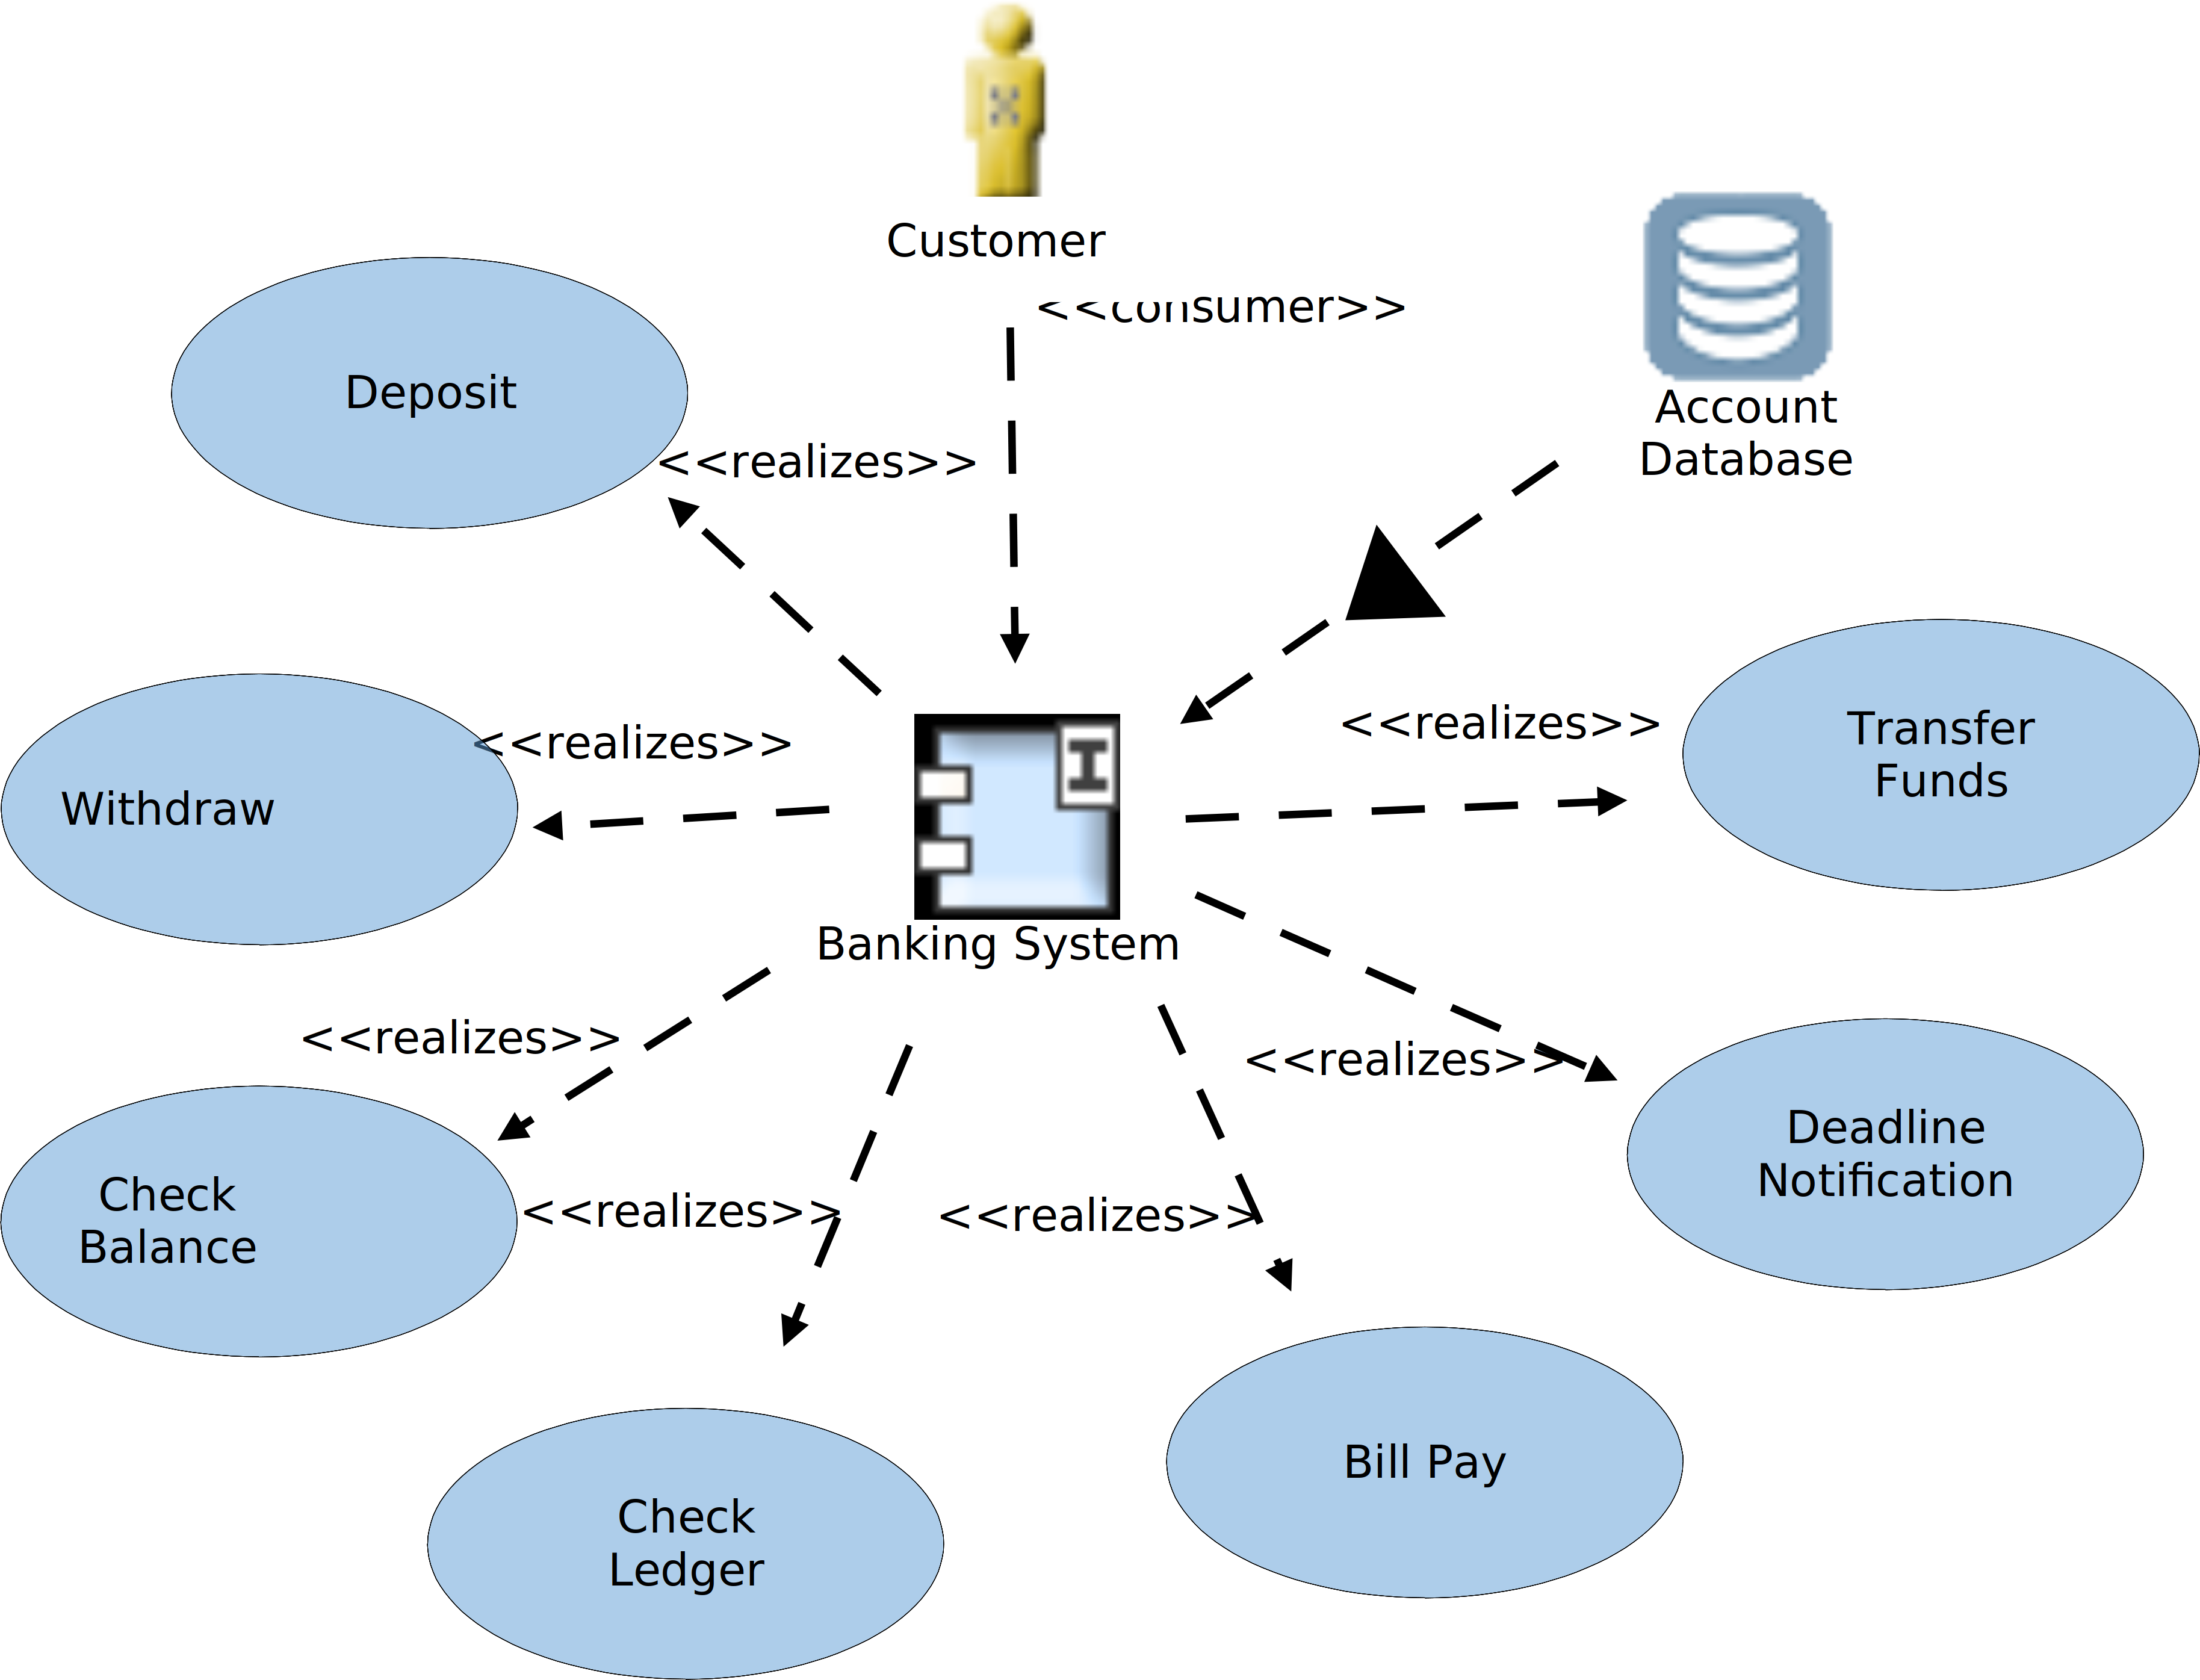
\includegraphics[width=\textwidth]{context_model.png}
  \caption{Context model diagram of the system}
\end{figure}

\appendix

\section{Screenshots}

\begin{figure}[H]
  \centering
    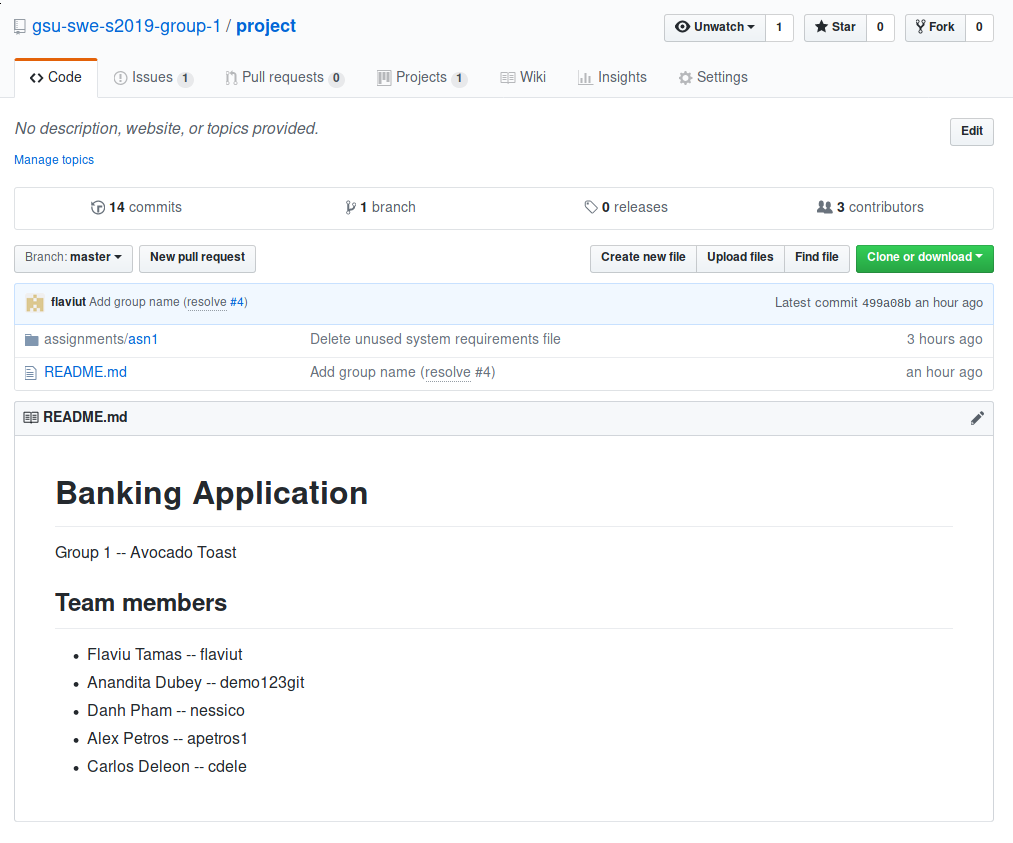
\includegraphics[width=\textwidth]{github_readme.png}
  \caption{Screenshot of our group's GitHub readme}
\end{figure}

\begin{figure}[H]
  \centering
    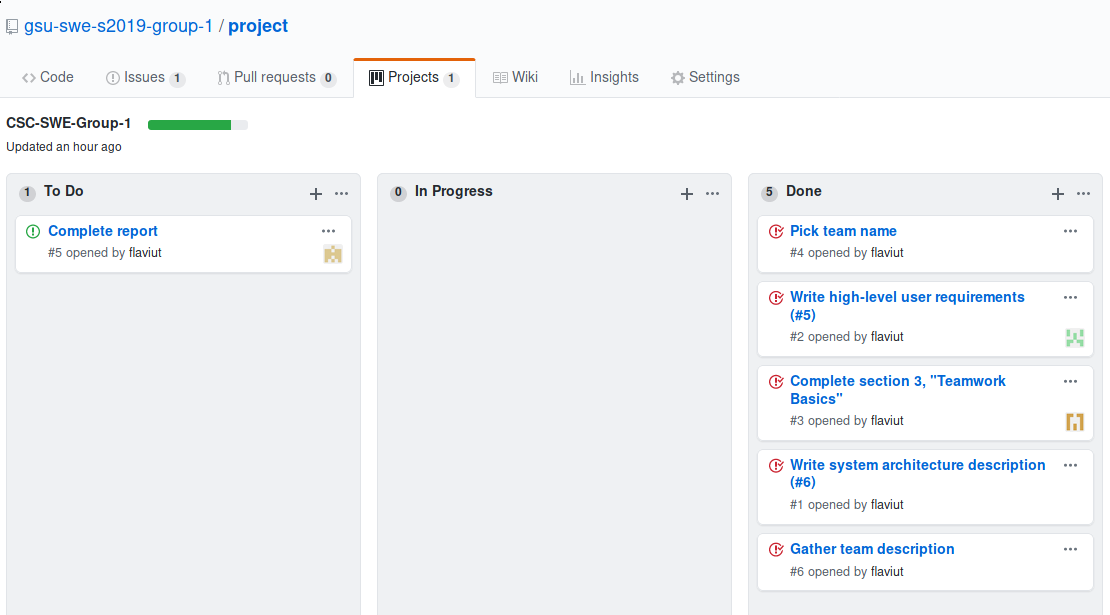
\includegraphics[width=\textwidth]{github_project.png}
  \caption{Screenshot of our group's Kanban board}
\end{figure}

\end{document}
